\chapter{Methodology}
\label{ch:methodology}

\section{A figure}
\label{sec:figure}

The figure below is a real PNG in \texttt{images/}. Dragging that file from
the explorer into the editor should insert a block just like this one, with
the caption and label filled in from the file name.

\begin{figure}[ht]
    \centering
    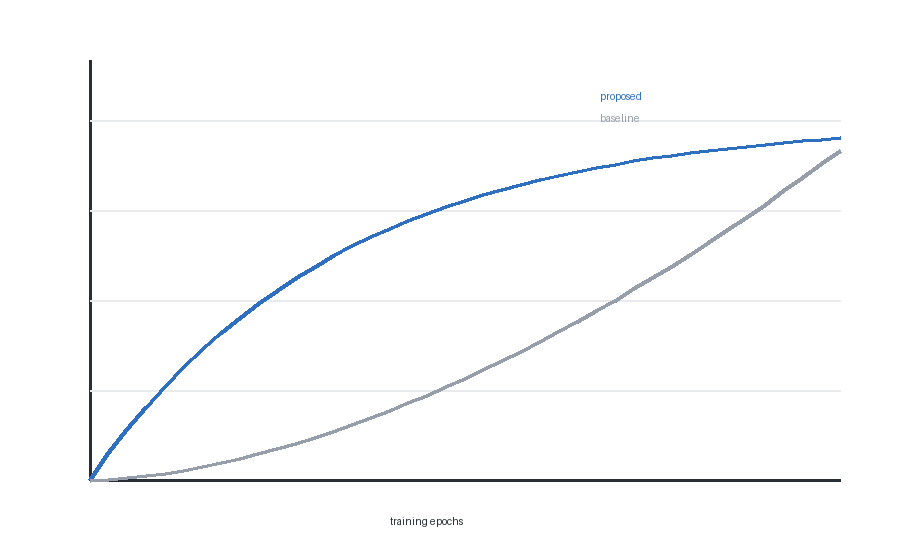
\includegraphics[width=0.75\textwidth]{images/convergence.png}
    \caption{Convergence of the proposed method against the baseline.}
    \label{fig:convergence}
\end{figure}

Figure~\ref{fig:convergence} is referenced here, which is what makes the
\texttt{listoffigures} entry and the page number appear correctly after the
second pass.

\section{A table}
\label{sec:table}

\begin{table}[ht]
    \centering
    \begin{tabular}{lrr}
        \toprule
        Method & Accuracy & Time (s) \\
        \midrule
        Baseline          & 0.81 & 12.4 \\
        Proposed          & 0.94 & 15.1 \\
        Proposed (tuned)  & 0.96 & 18.7 \\
        \bottomrule
    \end{tabular}
    \caption{Results on the held-out set.}
    \label{tab:results}
\end{table}

Table~\ref{tab:results} is discussed in Chapter~\ref{ch:results}.
